\documentclass[a4paper, notitlepage]{extreport}
\usepackage{lipsum} % for testing
\usepackage{titling}
\usepackage{authblk}
\usepackage{xcolor}
\usepackage{graphicx}
\usepackage{textcomp} % for euros

\providecommand{\tightlist}{%
  \setlength{\itemsep}{0pt}\setlength{\parskip}{0pt}}

% margins
\usepackage[a4paper, margin=2.5cm]{geometry}


% spacing
\usepackage{setspace}
\onehalfspacing

\usepackage{amsmath} % align equations
% fonts
\usepackage{mathspec}
\usepackage{fontspec}
\setmonofont[Scale=MatchLowercase]{JetBrains Mono Regular}
\setallmainfonts(Digits,Latin){XCharter}
\setmainfont{XCharter}

% misc
\usepackage{type1cm}
\usepackage{lettrine} % add large first letters
\usepackage{natbib} % bib management, maybe switch for biblatex
\usepackage{multicol} % for bib and definitions

% Create \R{}
\newcommand{\R}{\textbf{\textsf{R}}}

% better paragraph indents
\edef\restoreparindent{\parindent=\the\parindent\relax}
\usepackage{parskip}
\restoreparindent

% captions
\usepackage[font=footnotesize,
            labelfont=bf,
            textfont=it,
            margin=.5cm
            ]{caption}
% Figure names
\renewcommand{\figurename}{Fig.}

% style
\usepackage{fancyhdr}
\usepackage{lastpage}


% custom rule lines for headers/footersr
\newcommand*\ruleline[1]{\par\noindent\raisebox{.8ex}{\makebox[\linewidth]{\hrulefill\hspace{1ex}\raisebox{-.6ex}{#1}\hspace{1ex}}}}

\newcommand*\rulelinel[1]{\par\noindent\raisebox{.8ex}{\makebox[\linewidth]{\hrulefill\hspace{1ex}\raisebox{-.6ex}{#1}\hspace{1ex}\hrulefill}}}

\fancypagestyle{newchapter}{%
\fancyhf{} % clear all header and footer fields
\renewcommand{\headrulewidth}{0pt}
\renewcommand{\footrulewidth}{0pt}
\rfoot{\ruleline{\fontsize{9}{9}\bfseries Page \thepage\ of \pageref{LastPage}}}
}

\fancypagestyle{firststyle}{
\fancyhf{}
\renewcommand{\headrulewidth}{0pt}
\setlength{\headsep}{10pt}
\renewcommand{\footrulewidth}{0pt}
\lhead{\rulelinel{\fontsize{9}{9}\bfseries \leftmark}}
\rfoot{\ruleline{\fontsize{9}{9}\bfseries Page \thepage\ of \pageref{LastPage}}}
\setlength{\footskip}{20pt}
}

\fancypagestyle{preamble}{
\fancyhf{}
\renewcommand{\headrulewidth}{0pt}
\lfoot{\rulelinel{\fontsize{9}{9}\bfseries \thepage}}
}

\fancypagestyle{ack}{
\fancyhf{}
\renewcommand{\headrulewidth}{0.4pt}
\lfoot{\rulelinel{\fontsize{9}{9}\bfseries \thepage}}
}

\fancypagestyle{empty}{
\fancyhf{}
\renewcommand{\headrulewidth}{.4pt}
\renewcommand{\footrulewidth}{.4pt}
}


% For professional looking tables
\usepackage{booktabs} 

% Hyperlinks
\definecolor{darkblue}{rgb}{0.0,0.0,0.4}
\definecolor{darkred}{rgb}{0.5,0.0,0.0}
\usepackage{hyperref}
\hypersetup{
    colorlinks = true,
    linkcolor = darkred,
    anchorcolor = darkred,
    citecolor = darkred,
    urlcolor = darkblue
}
\urlstyle{rm}

% Table of content settings
\setcounter{tocdepth}{2}
\setcounter{secnumdepth}{2}
\usepackage{tocbasic}
\addtotoclist[report.cls]{toc}
\renewcommand*{\tableofcontents}{\listoftoc[{\contentsname}]{toc}}% ToC under control of tocbasic
\AfterTOCHead[toc]{\thispagestyle{preamble}\pagestyle{ack}}
\AfterStartingTOC[toc]{\clearpage}

% change chapters
\usepackage{titlesec}

\titleformat{\chapter}
{\Large\bfseries}
{}
{0.5em}
{\titlerule\, \thechapter. \thispagestyle{newchapter}}

\titleformat{name=\chapter,numberless}
{\Large\bfseries}
{}
{0.5em}
{\titlerule\enspace \thispagestyle{preamble}}
[]

% sections
\titleformat{\section}
{\large\bfseries}
{}
{0.5em}
{\thesection. }
[]

\titleformat{name=\section,numberless}
{\large\bfseries}
{}
{0.5em}
{}
[]

% subsections
\titleformat{\subsection}
{\normalsize\itshape\bfseries}
{}
{0.5em}
{\thesubsection. }
[]

% subsections
\titleformat{\subsubsection}
{\small\itshape}
{}
{0.5em}
{\thesubsubsection. }
[]

\providecommand{\keywords}[1]{\footnotesize\textbf{\textit{Keywords:}} #1}

\newcommand{\copyrightfont}{\linespread{1}\normalfont\rmfamily\fontsize{7}{8}\selectfont}
\renewcommand\Authfont{\normalfont\sffamily\bfseries\fontsize{11}{11}\selectfont}
\newcommand{\ackfont}{\rmfamily\bfseries\fontsize{9}{9}\selectfont}
\newcommand{\datesfont}{\linespread{1}\normalfont\sffamily\fontsize{10}{8}\selectfont}
\newcommand{\titlefont}{\linespread{1}\normalfont\rmfamily\fontsize{22pt}{24pt}\selectfont}

% bib
\setlength{\bibsep}{10pt}
\renewcommand*{\bibfont}{\normalfont\rmfamily\fontsize{9.5}{10}\selectfont} % set font to be sans serif

\pagestyle{firststyle}

\renewcommand*\footnoterule{}

% custom bib
\usepackage{etoolbox}
\usepackage{relsize}
\patchcmd{\thebibliography}
  {\list}
  {\begin{multicols}{2}\smaller\list}
  {}
  {}
\appto{\endthebibliography}{\end{multicols}}

\appto\appendix{\addtocontents{toc}{\protect\setcounter{tocdepth}{1}}}

% reinstate the correct level for list of tables and figures
\appto\listoffigures{\addtocontents{lof}{\protect\setcounter{tocdepth}{1}}}
\appto\listoftables{\addtocontents{lot}{\protect\setcounter{tocdepth}{1}}}

\title{Title of Chapter Based Report}
\author{Your Name}

\begin{document}
\pagenumbering{Roman}

    \maketitle

{\copyrightfont\author{Your Name}}

\date{}
    \thispagestyle{empty}
    \vskip 50pt
  \begin{abstract}
      \centering\begin{minipage}{\dimexpr\paperwidth-10cm}
          \hrule
          \vskip 5pt
    \lipsum[1-1]
    \vskip 5pt
    \hrule
    \vskip 10pt
\keywords{testing; testing; testing}
\end{minipage}
  \end{abstract}

\vskip 12pt

{\copyrightfont\centerline{\bfseries In Partial Fulfillment of the Requirements for the Degree of}}
{\copyrightfont\centerline{\bfseries Data Analytics and Society PhD}}
\centerline{
\includegraphics[width = 100mm]{./template/uolLogo.png}}
\newpage

\tableofcontents

\listoffigures

\listoftables

\newpage

\pagenumbering{arabic}

\chapter{Introduction}

\lipsum[1-2]

\hypertarget{example-plot}{%
\subsection{Example plot}\label{example-plot}}

Reference to a plot Figure \ref{fig:plot}.

\lipsum[1-1]

\begin{figure}[tb]

{\centering 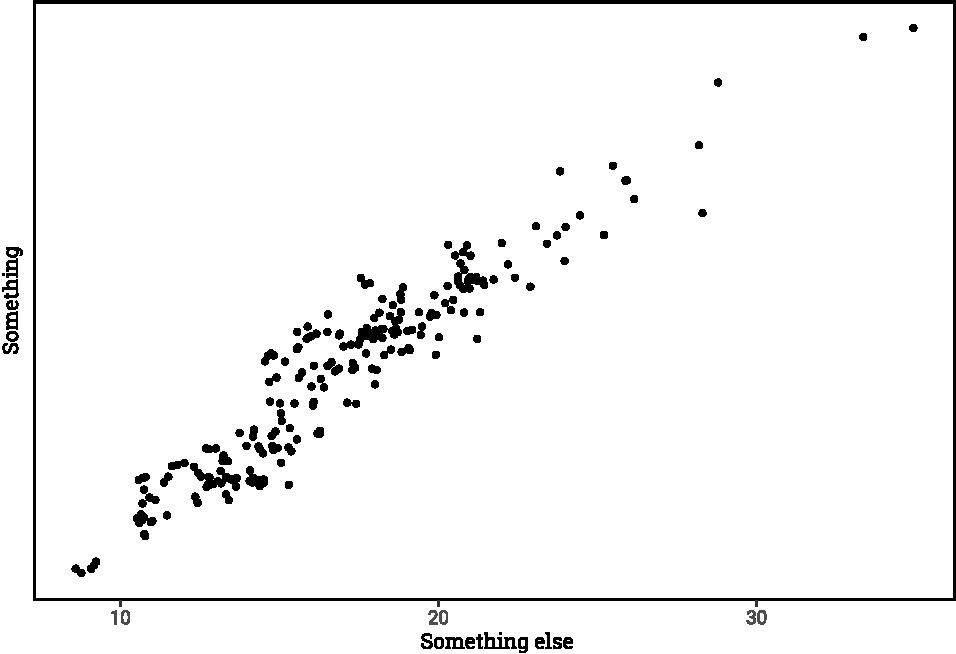
\includegraphics[width=.75\linewidth]{skeleton_files/figure-latex/plot-1} 

}

\caption{Example plot showing default ggplot2 theme}\label{fig:plot}
\end{figure}

\lipsum

\begin{table}

\caption{\label{tab:table_1}Test caption}
\centering
\fontsize{9}{11}\selectfont
\begin{tabular}[t]{lccccccccc}
\toprule
\textbf{ } & \textbf{mpg} & \textbf{cyl} & \textbf{disp} & \textbf{hp} & \textbf{drat} & \textbf{wt} & \textbf{qsec} & \textbf{vs} & \textbf{am}\\
\midrule
Mazda RX4 & 21.0 & 6 & 160.0 & 110 & 3.90 & 2.62 & 16.46 & 0 & 1\\
Mazda RX4 Wag & 21.0 & 6 & 160.0 & 110 & 3.90 & 2.88 & 17.02 & 0 & 1\\
Datsun 710 & 22.8 & 4 & 108.0 & 93 & 3.85 & 2.32 & 18.61 & 1 & 1\\
Hornet 4 Drive & 21.4 & 6 & 258.0 & 110 & 3.08 & 3.21 & 19.44 & 1 & 0\\
Hornet Sportabout & 18.7 & 8 & 360.0 & 175 & 3.15 & 3.44 & 17.02 & 0 & 0\\
Valiant & 18.1 & 6 & 225.0 & 105 & 2.76 & 3.46 & 20.22 & 1 & 0\\
Duster 360 & 14.3 & 8 & 360.0 & 245 & 3.21 & 3.57 & 15.84 & 0 & 0\\
Merc 240D & 24.4 & 4 & 146.7 & 62 & 3.69 & 3.19 & 20.00 & 1 & 0\\
Merc 230 & 22.8 & 4 & 140.8 & 95 & 3.92 & 3.15 & 22.90 & 1 & 0\\
Merc 280 & 19.2 & 6 & 167.6 & 123 & 3.92 & 3.44 & 18.30 & 1 & 0\\
Merc 280C & 17.8 & 6 & 167.6 & 123 & 3.92 & 3.44 & 18.90 & 1 & 0\\
Merc 450SE & 16.4 & 8 & 275.8 & 180 & 3.07 & 4.07 & 17.40 & 0 & 0\\
Merc 450SL & 17.3 & 8 & 275.8 & 180 & 3.07 & 3.73 & 17.60 & 0 & 0\\
Merc 450SLC & 15.2 & 8 & 275.8 & 180 & 3.07 & 3.78 & 18.00 & 0 & 0\\
Cadillac Fleetwood & 10.4 & 8 & 472.0 & 205 & 2.93 & 5.25 & 17.98 & 0 & 0\\
\bottomrule
\end{tabular}
\end{table}
\chapter{Literature Review}

\lipsum
\chapter{Methodology}

\lipsum
\chapter{Results}

\lipsum
\chapter{Discussion}

\lipsum

\nocite{tidyverse,devtools,ggthemes,kableExtra,scales,cowplot,bibtex,benchmarkme,showtext,data.table}
\noindent

\rule{2cm}{0.4pt}

Word Count: Path does not exist or is not a file: *.tex

\bibliographystyle{jss}
\linespread{1}
\bibliography{bib/kbib.bib, bib/rbib.bib}

\appendix
\chapter{Environment and Functions}

\begin{verbatim}
Machine:     
\end{verbatim}

\begin{verbatim}
[1] "AMD Ryzen 7 3700X 8-Core Processor"
\end{verbatim}

\begin{verbatim}
Num cores:   
\end{verbatim}

\begin{verbatim}
[1] 16
\end{verbatim}

\begin{verbatim}
Num threads: 
\end{verbatim}

\begin{verbatim}
[1] 16
\end{verbatim}

\begin{verbatim}
RAM:         
\end{verbatim}

\begin{verbatim}
33.7 GB
\end{verbatim}

\begin{verbatim}
R version 4.0.2 (2020-06-22)
Platform: x86_64-pc-linux-gnu (64-bit)
Running under: Arch Linux

Matrix products: default
BLAS:   /usr/lib/libopenblasp-r0.3.10.so
LAPACK: /usr/lib/liblapack.so.3.9.0

attached base packages:
[1] stats     graphics  grDevices utils     datasets  methods   base     

other attached packages:
 [1] data.table_1.12.8 showtext_0.8-1    showtextdb_3.0    sysfonts_0.8.1   
 [5] benchmarkme_1.0.4 bibtex_0.4.2.2    cowplot_1.0.0     scales_1.1.1     
 [9] kableExtra_1.1.0  ggthemes_4.2.0    forcats_0.5.0     stringr_1.4.0    
[13] dplyr_1.0.0       purrr_0.3.4       readr_1.3.1       tidyr_1.1.0      
[17] tibble_3.0.1      ggplot2_3.3.2     tidyverse_1.3.0   cjrmd_0.0.0.9000 
[21] devtools_2.3.0    usethis_1.6.1     pacman_0.5.1     
\end{verbatim}


\end{document}
